%TODO: Use LaTeX_Header
\documentclass{article}
\iffalse
This file is protected by Copyright. Please refer to the COPYRIGHT file
distributed with this source distribution.

This file is part of OpenCPI <http://www.opencpi.org>

OpenCPI is free software: you can redistribute it and/or modify it under the
terms of the GNU Lesser General Public License as published by the Free Software
Foundation, either version 3 of the License, or (at your option) any later
version.

OpenCPI is distributed in the hope that it will be useful, but WITHOUT ANY
WARRANTY; without even the implied warranty of MERCHANTABILITY or FITNESS FOR A
PARTICULAR PURPOSE. See the GNU Lesser General Public License for more details.

You should have received a copy of the GNU Lesser General Public License along
with this program. If not, see <http://www.gnu.org/licenses/>.
\fi

\author{} % Force author to be blank
%----------------------------------------------------------------------------------------
% Paper size, orientation and margins
%----------------------------------------------------------------------------------------
\usepackage{geometry}
\geometry{
	letterpaper,			% paper type
	portrait,				% text direction
	left=.75in,				% left margin
	top=.75in,				% top margin
	right=.75in,			% right margin
	bottom=.75in			% bottom margin
 }
%----------------------------------------------------------------------------------------
% Header/Footer
%----------------------------------------------------------------------------------------
\usepackage{fancyhdr} \pagestyle{fancy} % required for fancy headers
\renewcommand{\headrulewidth}{0.5pt}
\renewcommand{\footrulewidth}{0.5pt}
\rhead{\small{ANGRYVIPER Team}}
%----------------------------------------------------------------------------------------
% Appendix packages
%----------------------------------------------------------------------------------------
\usepackage[toc,page]{appendix}
%----------------------------------------------------------------------------------------
% Defined Commands & Renamed Commands
%----------------------------------------------------------------------------------------
\renewcommand{\contentsname}{Table of Contents}
\renewcommand{\listfigurename}{List of Figures}
\renewcommand{\listtablename}{List of Tables}
%----------------------------------------------------------------------------------------
% Various pacakges
%----------------------------------------------------------------------------------------
\usepackage{hyperref} % for linking urls and lists
\usepackage{graphicx} % for including pictures by file
\usepackage{listings} % for coding language styles
\usepackage{rotating} % for sideways table
\usepackage{pifont}   % for sideways table
\usepackage{pdflscape} % for landscape view
\usepackage{longtable}
%----------------------------------------------------------------------------------------
% Table packages
%----------------------------------------------------------------------------------------
\usepackage{tabularx} % c=center,l=left,r=right,X=fill
\usepackage{float}
\floatstyle{plaintop}
\usepackage[tableposition=top]{caption}
\newcolumntype{P}[1]{>{\centering\arraybackslash}p{#1}}
\newcolumntype{M}[1]{>{\centering\arraybackslash}m{#1}}
%----------------------------------------------------------------------------------------
% Block Diagram / FSM Drawings
%----------------------------------------------------------------------------------------
\usepackage{tikz}
\usetikzlibrary{shapes,arrows,fit,positioning}
\usetikzlibrary{automata} % used for the fsm
%----------------------------------------------------------------------------------------
% Colors Used
%----------------------------------------------------------------------------------------
\usepackage{colortbl}
\definecolor{blue}{rgb}{.7,.8,.9}
\definecolor{ceruleanblue}{rgb}{0.16, 0.32, 0.75}
\definecolor{drkgreen}{rgb}{0,0.6,0}
\definecolor{deepmagenta}{rgb}{0.8, 0.0, 0.8}
\definecolor{cyan}{rgb}{0.0,0.6,0.6}
\definecolor{maroon}{rgb}{0.5,0,0}

\usepackage{fancyvrb}

% used for identifying (and explaining in footnotes) OpenCPI non-component-spec properties
\renewcommand*{\thefootnote}{\fnsymbol{footnote}}

\usepackage{footmisc}
\usepackage{multirow}

%----------------------------------------------------------------------------------------
% Update the docTitle and docVersion per document
%----------------------------------------------------------------------------------------
\def\docTitle{Worker Data Sheet}
\def\docVersion{1.5}
%----------------------------------------------------------------------------------------
\date{Version \docVersion} % Force date to be blank and override date with version
%TODO: Why doesn't this use LaTeX_Header?
\def\snippetpath{../../../../../../doc/av/tex/snippets}
% Usage:
% \def\snippetpath{../../../../../doc/av/tex/snippets/}
% % Usage:
% \def\snippetpath{../../../../../doc/av/tex/snippets/}
% % Usage:
% \def\snippetpath{../../../../../doc/av/tex/snippets/}
% \input{\snippetpath/includes}
% From then on, you can use "input" With no paths to get to "snippets"
% You also get all "major" snippets not part of the global LaTeX_Header
% NOTE: If not using the global LaTeX_Header, you need to
% \usepackage{ifthen} to use the \githubio macro

\hyphenation{ANGRY-VIPER} % Tell it where to hyphenate
\hyphenation{Cent-OS} % Tell it where to hyphenate
\hyphenation{install-ation} % Tell it where to hyphenate

\newcommand{\todo}[1]{\textcolor{red}{TODO: #1}\PackageWarning{TODO:}{#1}} % To do notes
\newcommand{\code}[1]{\texttt{#1}} % For inline code snippet or command line
\newcommand{\sref}[1]{Section~\ref{#1}} % To quickly reference a section

% To quickly reference a versioned PDF on gitlab.io
\def\ocpiversion{develop}

% This gives a link to gitlab.io document. By default, it puts the filename.
% You can optionally change the link, e.g.
% \githubio{FPGA\_Vendor\_Tools\_Installation\_Guide.pdf} vs.
% \githubio[\textit{FPGA Vendor Tools Installation Guide}]{FPGA\_Vendor\_Tools\_Installation\_Guide.pdf}
% or if you want the raw ugly URL to come out, \githubioURL{FPGA_Vendor_Tools_Installation_Guide.pdf}
\newcommand{\githubio}[2][]{% The default is for FIRST param!
\href{http://opencpi.gitlab.io/releases/\ocpiversion/docs/#2}{\ifthenelse{\equal{#1}{}}{\texttt{#2}}{#1}}}
\newcommand{\gitlabcom}[2][]{% The default is for FIRST param!
\href{http://gitlab.com/opencpi/#2}{\ifthenelse{\equal{#1}{}}{\texttt{#2}}{#1}}}
\newcommand{\githubioURL}[1]{\url{http://opencpi.gitlab.io/releases/\ocpiversion/docs/#1}}
% Lastly, if you want a SINGLE leading path stripped, e.g. assets/X.pdf => X.pdf:
\newcommand{\githubioFlat}[1]{%
\StrBehind{#1}{/}[\den]%
\href{http://opencpi.gitlab.io/releases/\ocpiversion/docs/#1}{\texttt{\den}}%
}

% Fix import paths
\makeatletter
\def\input@path{{\snippetpath/}}
\makeatother

% From then on, you can use "input" With no paths to get to "snippets"
% You also get all "major" snippets not part of the global LaTeX_Header
% NOTE: If not using the global LaTeX_Header, you need to
% \usepackage{ifthen} to use the \githubio macro

\hyphenation{ANGRY-VIPER} % Tell it where to hyphenate
\hyphenation{Cent-OS} % Tell it where to hyphenate
\hyphenation{install-ation} % Tell it where to hyphenate

\newcommand{\todo}[1]{\textcolor{red}{TODO: #1}\PackageWarning{TODO:}{#1}} % To do notes
\newcommand{\code}[1]{\texttt{#1}} % For inline code snippet or command line
\newcommand{\sref}[1]{Section~\ref{#1}} % To quickly reference a section

% To quickly reference a versioned PDF on gitlab.io
\def\ocpiversion{develop}

% This gives a link to gitlab.io document. By default, it puts the filename.
% You can optionally change the link, e.g.
% \githubio{FPGA\_Vendor\_Tools\_Installation\_Guide.pdf} vs.
% \githubio[\textit{FPGA Vendor Tools Installation Guide}]{FPGA\_Vendor\_Tools\_Installation\_Guide.pdf}
% or if you want the raw ugly URL to come out, \githubioURL{FPGA_Vendor_Tools_Installation_Guide.pdf}
\newcommand{\githubio}[2][]{% The default is for FIRST param!
\href{http://opencpi.gitlab.io/releases/\ocpiversion/docs/#2}{\ifthenelse{\equal{#1}{}}{\texttt{#2}}{#1}}}
\newcommand{\gitlabcom}[2][]{% The default is for FIRST param!
\href{http://gitlab.com/opencpi/#2}{\ifthenelse{\equal{#1}{}}{\texttt{#2}}{#1}}}
\newcommand{\githubioURL}[1]{\url{http://opencpi.gitlab.io/releases/\ocpiversion/docs/#1}}
% Lastly, if you want a SINGLE leading path stripped, e.g. assets/X.pdf => X.pdf:
\newcommand{\githubioFlat}[1]{%
\StrBehind{#1}{/}[\den]%
\href{http://opencpi.gitlab.io/releases/\ocpiversion/docs/#1}{\texttt{\den}}%
}

% Fix import paths
\makeatletter
\def\input@path{{\snippetpath/}}
\makeatother

% From then on, you can use "input" With no paths to get to "snippets"
% You also get all "major" snippets not part of the global LaTeX_Header
% NOTE: If not using the global LaTeX_Header, you need to
% \usepackage{ifthen} to use the \githubio macro

\hyphenation{ANGRY-VIPER} % Tell it where to hyphenate
\hyphenation{Cent-OS} % Tell it where to hyphenate
\hyphenation{install-ation} % Tell it where to hyphenate

\newcommand{\todo}[1]{\textcolor{red}{TODO: #1}\PackageWarning{TODO:}{#1}} % To do notes
\newcommand{\code}[1]{\texttt{#1}} % For inline code snippet or command line
\newcommand{\sref}[1]{Section~\ref{#1}} % To quickly reference a section

% To quickly reference a versioned PDF on gitlab.io
\def\ocpiversion{develop}

% This gives a link to gitlab.io document. By default, it puts the filename.
% You can optionally change the link, e.g.
% \githubio{FPGA\_Vendor\_Tools\_Installation\_Guide.pdf} vs.
% \githubio[\textit{FPGA Vendor Tools Installation Guide}]{FPGA\_Vendor\_Tools\_Installation\_Guide.pdf}
% or if you want the raw ugly URL to come out, \githubioURL{FPGA_Vendor_Tools_Installation_Guide.pdf}
\newcommand{\githubio}[2][]{% The default is for FIRST param!
\href{http://opencpi.gitlab.io/releases/\ocpiversion/docs/#2}{\ifthenelse{\equal{#1}{}}{\texttt{#2}}{#1}}}
\newcommand{\gitlabcom}[2][]{% The default is for FIRST param!
\href{http://gitlab.com/opencpi/#2}{\ifthenelse{\equal{#1}{}}{\texttt{#2}}{#1}}}
\newcommand{\githubioURL}[1]{\url{http://opencpi.gitlab.io/releases/\ocpiversion/docs/#1}}
% Lastly, if you want a SINGLE leading path stripped, e.g. assets/X.pdf => X.pdf:
\newcommand{\githubioFlat}[1]{%
\StrBehind{#1}{/}[\den]%
\href{http://opencpi.gitlab.io/releases/\ocpiversion/docs/#1}{\texttt{\den}}%
}

% Fix import paths
\makeatletter
\def\input@path{{\snippetpath/}}
\makeatother

\title{\docTitle}
\lhead{\small{\docTitle}}

\def\comp{dig\_radio\_ctrlr\_fmcomms\_2\_3}
\def\Comp{FMCOMMS2/3 Digital Radio Controller}
\graphicspath{ {figures/} }

\begin{document}

\section*{Summary - FMCOMMS2/3 Digital Radio Controller Worker}
\begin{longtable}{|p{\dimexpr0.5\textwidth-2\tabcolsep\relax}
                  |p{\dimexpr0.5\textwidth-2\tabcolsep\relax}|}
	\hline
	\rowcolor{blue}
	                  &                                        \\
	\hline
	Package Prefix    & ocpi.core \\
	\hline
	Component         & dig\_radio\_ctrlr \\
	\hline
	Name              & \comp                                  \\
	\hline
	Authoring Model   & rcc                                    \\
	\hline
	Version          & 1 \\
	\hline
	OpenCPI Release & v\docVersion ~ (released 4/2019) \\
	\hline
\end{longtable}

\begin{center}
  \textit{\textbf{Revision History}}
  \begin{longtable}{|p{\dimexpr0.15\textwidth-2\tabcolsep\relax}
                    |p{\dimexpr0.65\textwidth-2\tabcolsep\relax}
                    |p{\dimexpr0.2\textwidth-2\tabcolsep\relax}|}
    \hline
    \rowcolor{blue}
    \textbf{Revision} & \textbf{Description of Change} & \textbf{Date} \\
    \hline
    v1.5 & Initial Release & 4/2019 \\
    \hline
    \color{red}vdevelop & \item Worker updated to use latest No-OS 2018\_R2 release & N/A \\
    \hline
  \end{longtable}
\end{center}

\section{Block Diagrams}

  \begin{figure}[H]
  \centering
  \begin{tikzpicture}[% List of styles applied to all, to override specify on a case-by-case
      every node/.style={
        align=center,     % use this so that the "\\" for line break works
        minimum size=2cm  % creates space above and below text in rectangle
      },
      every edge/.style={draw,thick}
    ]
    \node[rectangle,ultra thick,draw=black,fill=blue](R2){Parameter Properties:
\verb+MAX_STRING_LENGTH_p+, \\
\verb+NUM_DATA_STREAM_IDS_p+,
\verb+NUM_DATA_STREAM_IDS_RX_p+,
\verb+NUM_DATA_STREAM_IDS_TX_p+, \\
\verb+DATA_STREAM_IDS_RX_p+,
\verb+DATA_STREAM_IDS_TX_p+, \\
\verb+MAX_NUM_DATA_STREAMS_RX_p+,
\verb+MAX_NUM_DATA_STREAMS_TX_p+, \\
\verb+MIN_ACHIEVABLE_RX_TUNING_FREQ_MHZ_p+,
\verb+MAX_ACHIEVABLE_RX_TUNING_FREQ_MHZ_p+, \\
\verb+MIN_ACHIEVABLE_RX_BANDWIDTH_3DB_MHZ_p+,
\verb+MAX_ACHIEVABLE_RX_BANDWIDTH_3DB_MHZ_p+, \\
\verb+MIN_ACHIEVABLE_RX_SAMPLING_RATE_MSPS_p+,
\verb+MAX_ACHIEVABLE_RX_SAMPLING_RATE_MSPS_p+, \\
\verb+IS_SUPPORTED_RX_SAMPLES_COMPLEX_p+,
\verb+IS_SUPPORTED_RX_SAMPLES_REAL_p+, \\
\verb+IS_SUPPORTED_RX_GAIN_MODE_AUTO_p+,
\verb+IS_SUPPORTED_RX_GAIN_MODE_MANUAL_p+, \\
\verb+MIN_ACHIEVABLE_TX_TUNING_FREQ_MHZ_p+,
\verb+MAX_ACHIEVABLE_TX_TUNING_FREQ_MHZ_p+, \\
\verb+MIN_ACHIEVABLE_TX_BANDWIDTH_3DB_MHZ_p+,
\verb+MAX_ACHIEVABLE_TX_BANDWIDTH_3DB_MHZ_p+, \\
\verb+MIN_ACHIEVABLE_TX_SAMPLING_RATE_MSPS_p+,
\verb+MAX_ACHIEVABLE_TX_SAMPLING_RATE_MSPS_p+, \\
\verb+IS_SUPPORTED_TX_SAMPLES_COMPLEX_p+,
\verb+IS_SUPPORTED_TX_SAMPLES_REAL_p+ \\
\verb+FMCOMMS_NUM_p+\textsuperscript{\ref{nonspecprop}} \\ \\
\Comp \\};
    \node[rectangle,draw=white,fill=white](R5)[above= of R2]{
      Non-parameter Properties: \verb+request_config_lock+,
      \verb+config_locks+, \verb+unlock_config_lock+,
      \verb+unlock_all+, \\ \verb+data_stream_is_enabled+, \\
      \verb+direction_readback+, \\
      \verb+tuning_freq_MHz+,
      \verb+bandwidth_3dB_MHz+, \verb+sampling_rate_Msps+,
      \verb+samples_are_complex+, \\ \verb+valid_values_tuning_freq_MHz+, \\
      \verb+valid_values_bandwidth_3dB_MHz+, \\
      \verb+valid_values_sampling_rate_Msps+, \\
      \verb+valid_values_samples_are_complex+, \\
      \verb+gain_mode_readback+\textsuperscript{\ref{nonspecprop}},
      \verb+gain_mode_dB+\textsuperscript{\ref{nonspecprop}}, \\
      \verb+valid_values_gain_mode+\textsuperscript{\ref{nonspecprop}},
      \verb+valid_values_gain_dB+\textsuperscript{\ref{nonspecprop}}, \\
      \verb+app_inst_name_TX0_qdac+\textsuperscript{\ref{nonspecprop}},
      \verb+app_inst_name_TX0_complex_mixer+\textsuperscript{\ref{nonspecprop}},
      \verb+app_inst_name_TX0_cic_int+\textsuperscript{\ref{nonspecprop}}, \\
      \verb+app_inst_name_TX1_qdac+\textsuperscript{\ref{nonspecprop}},
      \verb+app_inst_name_TX1_complex_mixer+\textsuperscript{\ref{nonspecprop}},
      \verb+app_inst_name_TX1_cic_int+\textsuperscript{\ref{nonspecprop}}, \\
      \verb+app_inst_name_RX0_qadc+\textsuperscript{\ref{nonspecprop}},
      \verb+app_inst_name_RX0_complex_mixer+\textsuperscript{\ref{nonspecprop}},
      \verb+app_inst_name_RX0_cic_dec+\textsuperscript{\ref{nonspecprop}}, \\
      \verb+app_inst_name_RX1_qadc+\textsuperscript{\ref{nonspecprop}},
      \verb+app_inst_name_RX1_complex_mixer+\textsuperscript{\ref{nonspecprop}},
      \verb+app_inst_name_RX1_cic_dec+\textsuperscript{\ref{nonspecprop}}, \\
      \verb+bist_loopback+\textsuperscript{\ref{nonspecprop}}
      };
    \path[->]
    (R2)edge [] node [] {} (R5)
    (R5)edge [] node [] {} (R2)
    ;
  \end{tikzpicture}
    \caption{Worker Block Diagram.}
  \end{figure}
\footnotetext[1]{\label{nonspecprop}indicates a non-spec property, i.e. one declared in the OWD}

\tableofcontents

\listoffigures

\section{Functionality}

  This worker implements the dig\_radio\_ctrlr component
  spec\cite{dig_radio_ctrlr_comp_datasheet} for the
  following Analog Devices FMC cards. The worker has a build configuration
  specific to each card.
  \begin{itemize}
    \item FMCOMMS2 Software Defined Radio card
      (2.4 GHz Optimized)\cite{fmcomms2_website}
    \item FMCOMMS3 wideband Software Defined Radio
      card\cite{fmcomms3_website}
  \end{itemize}

  \begin{center}
    \begin{figure}[h]
      \centering\captionsetup{type=figure}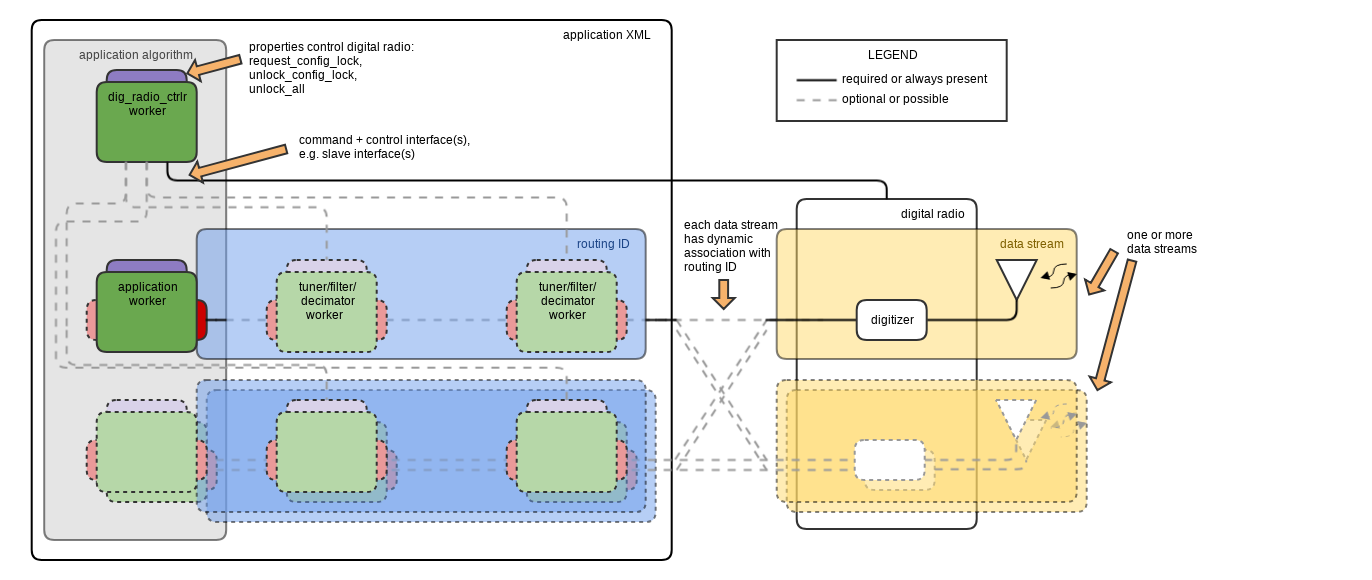
\includegraphics[scale=0.42]{dig_radio_ctrlr}
      \captionof{figure}{Digital Radio Controller - Major Concepts and Intended Usage.}
      \label{fig:blockdiagram}
    \end{figure}
  \end{center}

  \subsection{Implementation Details}
    \subsubsection{Slave Interfaces}
      This worker has a single slave interface to the ad9361\_config.hdl worker.
      This worker also potentially accesses properties of workers specified in
      the following \comp.rcc properties:
      \begin{itemize}
        \item \verb+app_inst_name_TX0_qdac+\textsuperscript{\ref{nonspecprop}}
        \item \verb+app_inst_name_TX0_complex_mixer+\textsuperscript{\ref{nonspecprop}}
        \item \verb+app_inst_name_TX0_cic_int+\textsuperscript{\ref{nonspecprop}}
        \item \verb+app_inst_name_TX1_qdac+\textsuperscript{\ref{nonspecprop}}
        \item \verb+app_inst_name_TX1_complex_mixer+\textsuperscript{\ref{nonspecprop}}
        \item \verb+app_inst_name_TX1_cic_int+\textsuperscript{\ref{nonspecprop}}
        \item \verb+app_inst_name_RX0_qadc+\textsuperscript{\ref{nonspecprop}}
        \item \verb+app_inst_name_RX0_complex_mixer+\textsuperscript{\ref{nonspecprop}}
        \item \verb+app_inst_name_RX0_cic_dec+\textsuperscript{\ref{nonspecprop}}
        \item \verb+app_inst_name_RX1_qadc+\textsuperscript{\ref{nonspecprop}}
        \item \verb+app_inst_name_RX1_complex_mixer+\textsuperscript{\ref{nonspecprop}}
        \item \verb+app_inst_name_RX1_cic_dec+\textsuperscript{\ref{nonspecprop}}
      \end{itemize}
\footnotetext[1]{\label{nonspecprop}indicates a non-spec property, i.e. one declared in the OWD}
      If any of these string properties have a value that is an empty string,
      no access is performed.
      The workers specified in the string properties are accessed via the ACI
      functions\cite{ocpi_app_guide}, e.g. setProperty().

    \subsubsection{Supporting C++ Classes}
      See the component spec
      datasheet \cite{dig_radio_ctrlr_comp_datasheet}
      for a description of the supporting base classes.
      The \\ RadioCtrlrFMCOMMS2TuneResamp and
      RadioCtrlrFMCOMMS3TuneResamp classes inherit from the
      RadioCtrlrNoOSTuneResamp class which is
      a software wrapper for Analog Device's No-OS software
      library\cite{no_os}.
      The version of No-OS used is GitHub commit ID
      8c52aa42e74841e3975a6f33cc5303ed2a670124 \cite{no_os_8c52aa42e74841e3975a6f33cc5303ed2a670124}.
      No-OS provides command and control of the FMCOMMS2/3's AD9361
      RF transceiver IC\cite{ad9361} via an
      API which ultimately controls SPI writes to the
      AD9361 register
      set. Note that the \comp.rcc worker does not currently
      expose all of the
      functionality
      of No-OS, as opposed to
      ad9361\_config\_proxy.rcc\cite{ad9361_config_proxy_datasheet}.
    If desired, doxygen documentation can be generated for all
    of the supporting classes in the dig\_radio\_ctlr\_fmcomms\_2\_3.rcc
    directory. Doxygen and
    either firefox or make and evince
    must be installed. To generate
    the documentation, run the following commands from the
    dig\_radio\_ctrlr\_fmcomms\_2\_3.rcc directory:
    \lstset{language=bash, backgroundcolor=\color{lightgray}, columns=flexible, breaklines=true, prebreak=\textbackslash, basicstyle=\ttfamily, showstringspaces=false,upquote=true, aboveskip=\baselineskip, belowskip=\baselineskip}
    \begin{lstlisting}
cd ./supporting/
doxygen
    \end{lstlisting}
The generated HTML documentation can be viewed via:
    \begin{lstlisting}
firefox ./html/index.html
    \end{lstlisting}
The generated PDF documentation can be viewed via:
    \begin{lstlisting}
make -C ./latex/
evince ./latex/refman.pdf
    \end{lstlisting}



  \subsection{Data Streams}
    See the component spec datasheet for
    \textit{data stream}, \textit{data stream ID}
    and
    \textit{data stream type}
    concepts and definitions\cite{dig_radio_ctrlr_comp_datasheet}.
    This worker has the following \textit{data stream IDs}, each of which
    corresponds to an SMA connector on the FMCOMMS2/3 PCB:
    \begin{itemize}
      \item SMA\_RX1A (can be configured for only the RX \textit{data stream type})
      \item SMA\_RX2A (can be configured for only the RX \textit{data stream type})
      \item SMA\_TX1A (can be configured for only the TX \textit{data stream type})
      \item SMA\_TX2A (can be configured for only the TX \textit{data stream type})
    \end{itemize}
    As stated in \cite{dig_radio_ctrlr_comp_datasheet},
    each \textit{data stream} entry for a \textit{config lock request} must
    refer to one of these \textit{data stream IDs} and a
    \textit{data stream type}.

  \subsection{Routing IDs}
    See the component spec datasheet for
    \textit{routing ID}
    concept and definition\cite{dig_radio_ctrlr_comp_datasheet}.
    The FMCOMMS2/3 cards support up to 4 simultaneously locked
    \textit{data streams} (2 RX and 2 TX),
    each of which is associated with a routing ID.
    In keeping with recommendation in
    \cite{dig_radio_ctrlr_comp_datasheet} for generic
    \textit{routing ID} format,
    this worker supports the following \textit{routing IDs}:
    \begin{itemize}
      \item RX0
      \item RX1
      \item TX0
      \item TX1
    \end{itemize}
    Each \textit{data stream} entry for a \textit{config lock request} must
    refer to one of these \textit{routing IDs}.
    Note that, when any of the following worker properties contain
    a non-empty string,
    the \textit{routing IDs} are associated with the application worker
    instance name specified in the string:
    \begin{itemize}
      \item \verb+app_inst_name_TX0_qdac+\textsuperscript{\ref{nonspecprop}}
      \item \verb+app_inst_name_TX0_complex_mixer+\textsuperscript{\ref{nonspecprop}}
      \item \verb+app_inst_name_TX0_cic_int+\textsuperscript{\ref{nonspecprop}}
      \item \verb+app_inst_name_TX1_qdac+\textsuperscript{\ref{nonspecprop}}
      \item \verb+app_inst_name_TX1_complex_mixer+\textsuperscript{\ref{nonspecprop}}
      \item \verb+app_inst_name_TX1_cic_int+\textsuperscript{\ref{nonspecprop}}
      \item \verb+app_inst_name_RX0_qadc+\textsuperscript{\ref{nonspecprop}}
      \item \verb+app_inst_name_RX0_complex_mixer+\textsuperscript{\ref{nonspecprop}}
      \item \verb+app_inst_name_RX0_cic_dec+\textsuperscript{\ref{nonspecprop}}
      \item \verb+app_inst_name_RX1_qadc+\textsuperscript{\ref{nonspecprop}}
      \item \verb+app_inst_name_RX1_complex_mixer+\textsuperscript{\ref{nonspecprop}}
      \item \verb+app_inst_name_RX1_cic_dec+\textsuperscript{\ref{nonspecprop}}
    \end{itemize}

  \subsection{Config Lock Requests}
    See the component spec datasheet for
    \textit{config lock request}
    concept and definition\cite{dig_radio_ctrlr_comp_datasheet}.
    Each \textit{data stream} entry for a \textit{config lock request} must
    refer to an
    aforementioned worker-specific \textit{data stream ID},
    \textit{data stream type}, and \textit{routing ID}.

\footnotetext[1]{\label{nonspecprop}indicates a non-spec property, i.e. one declared in the OWD}

  \subsection{Detailed Component Spec Property Descriptions}

    See the component spec detailed property
    description \cite{dig_radio_ctrlr_comp_datasheet}.

  \subsection{Detailed Non-Spec Property Descriptions}
    \label{sec:detailed_property_description}

    \subsubsection{Parameter Properties}
      \begin{itemize}
        \item \verb+FMCOMMS_NUM_p+\textsuperscript{\ref{nonspecprop}} property
          \begin{itemize}
            \item Valid values are 2 or 3. Used to allow worker to be parameterized
              for use with either FMCOMMS2 or FMCOMMS3.
              Application XML intended for use specific to FMCOMMS2/3 are expected
              to use the component selection XML attribute to restrict this
              value in order to
              enforce
              application requirements on intended FMCOMMS number.

          \end{itemize}
        \end{itemize}

    \subsubsection{Non-Parameter Properties - Current Value Reading}
    The
    \verb+gain_mode_readback+\textsuperscript{\ref{nonspecprop}} and
    \verb+gain_dB+\textsuperscript{\ref{nonspecprop}}
    sequence properties are used to read the current config value
    (locked or not) for each enabled \textit{data stream}. Each
    sequence element contains the current config value for an enabled
    \textit{data stream}. Worker implementations are expected to
    adjust this property's
    length such that it includes only enabled \textit{data streams}.
    If no \textit{data streams}
    are enabled, the sequence length is expected to be zero.

  \subsubsection{Non-Parameter Properties - Valid Values Reading}
  The
  \verb+valid_values_gain_mode+\textsuperscript{\ref{nonspecprop}} and
  \verb+valid_values_gain_dB+\textsuperscript{\ref{nonspecprop}}
  array properties indicate the current valid ranges of
  values for all \textit{data streams}/\textit{data stream type}
  combinations. Each array element contains the
  ranges for a single \textit{data stream} for a single
  \textit{data stream type}.
  It is expected that \textit{data streams} that can be configured for either
  RX or TX will have a separate entry for each possible
  \textit{data stream type}.
  Once a config is locked, it
  is intended that its valid ranges will only consist of a single value.

  \begin{center}
    \framebox{\parbox{0.8\linewidth}{\centering
      \textcolor{red}{WARNING:}
      % AV-4871
      The dig\_radio\_ctrlr\_fmcomms\_2\_3.rcc worker's
      valid\_values\_tuning\_freq\_MHz,
      valid\_values\_bandwidth\_3dB\_MHz,
      valid\_values\_sampling\_rate\_Msps,
      valid\_values\_gain\_mode\textsuperscript{\ref{nonspecprop}}, and
      valid\_values\_gain\_dB\textsuperscript{\ref{nonspecprop}}
      properties do not currently function as intended due to unimplemented
      functionality. Each of their valid\_values sequence member currently
      always has a sequence length of 0. Note that the
      valid\_values\_samples\_are\_complex\textsuperscript{\ref{nonspecprop}}
      property operates as intended. }}
  \end{center}

  \subsubsection{Application Instance Name Properties}
  As seen in \ref{fig:blockdiagram} and stated in
  \cite{dig_radio_ctrlr_comp_datasheet}, each \textit{routing ID}
  can be associated with one or more tuner/filter/resampler application workers.
  Each of the following string properties are used to associate a
  qadc, qdac, complex\_mixer, cic\_int, or cic\_dec worker
  with a \textit{routing ID} that falls under the command/control
  of the \comp{}.rcc worker.

  \begin{center}
    \framebox{\parbox{0.8\linewidth}{\centering
      \textcolor{red}{WARNING:}
      % AV-4838
      The phs\_inc property of any complex\_mixer application worker specified
      in the
      app\_inst\_name\_RX0\_complex\_mixer\textsuperscript{\ref{nonspecprop}}, \\
      app\_inst\_name\_RX1\_complex\_mixer\textsuperscript{\ref{nonspecprop}}, \\
      app\_inst\_name\_TX0\_complex\_mixer\textsuperscript{\ref{nonspecprop}}, or \\
      app\_inst\_name\_TX1\_complex\_mixer\textsuperscript{\ref{nonspecprop}} \\
      properties should \textit{not} be modified at runtime by the ACI. Doing so
      could
      erroneously invalidate \textit{config locks}. }}
  \end{center}

  \noindent
  Note that it is perfectly acceptable for an OAS to enforce the \verb+R+
  parameter
  property value of the cic\_int/cic\_dec workers for purposes of setting
  decimation/interpolation values. This is acceptable because the parameter
  property values cannot change at runtime.
  \begin{itemize}
    \item \verb+app_inst_name_TX0_qdac+\textsuperscript{\ref{nonspecprop}}
    \item \verb+app_inst_name_TX0_complex_mixer+\textsuperscript{\ref{nonspecprop}}
    \item \verb+app_inst_name_TX0_cic_int+\textsuperscript{\ref{nonspecprop}}
    \item \verb+app_inst_name_TX1_qdac+\textsuperscript{\ref{nonspecprop}}
    \item \verb+app_inst_name_TX1_complex_mixer+\textsuperscript{\ref{nonspecprop}}
    \item \verb+app_inst_name_TX1_cic_int+\textsuperscript{\ref{nonspecprop}}
    \item \verb+app_inst_name_RX0_qadc+\textsuperscript{\ref{nonspecprop}}
    \item \verb+app_inst_name_RX0_complex_mixer+\textsuperscript{\ref{nonspecprop}}
    \item \verb+app_inst_name_RX0_cic_dec+\textsuperscript{\ref{nonspecprop}}
    \item \verb+app_inst_name_RX1_qadc+\textsuperscript{\ref{nonspecprop}}
    \item \verb+app_inst_name_RX1_complex_mixer+\textsuperscript{\ref{nonspecprop}}
    \item \verb+app_inst_name_RX1_cic_dec+\textsuperscript{\ref{nonspecprop}}
  \end{itemize}

\footnotetext[1]{\label{nonspecprop}indicates a non-spec property, i.e. one declared in the OWD}

\begin{landscape}

\section{Worker Property Table(s)}
  For a detailed property description, see \ref{sec:detailed_property_description}. \\ \\

	\noindent Table \hypertarget{tab1}{1}: Component Spec Properties.
	\begin{scriptsize}
		\begin{longtable}{|p{5.16cm}|c|p{3.5cm}|p{3.4cm}|c|p{2.1cm}|p{3.75cm}|}
			\hline
			\rowcolor{blue}
			Name                                & Type   & Sequence & Array      & Accessibility       & Default & Description                                                                                \\
			\rowcolor{blue}
			                                    &        & Length   & Dimensions &                     &             &                                                                                            \\
			\hline
			\verb+MAX_STRING_LENGTH_p+ & UShort & -        & -          & Parameter           & 1024 \textsuperscript{\ref{nonspec}}  & Length of all string properties. \\
			\hline
			\verb+NUM_DATA_STREAM_IDS_p+           & UShort & -        & -          & Parameter           & 4 \textsuperscript{\ref{nonspec}}       & Total number of \textit{data stream IDs}. \\
			\hline
			\verb+NUM_DATA_STREAM_IDS_RX_p+        & UShort & -        & -          & Parameter           & 2 \textsuperscript{\ref{nonspec}}       & Total number of \textit{data stream IDs} that can be configured for RX streaming. \\
			\hline
			\verb+NUM_DATA_STREAM_IDS_TX_p+        & UShort & -        & -          & Parameter           & 2 \textsuperscript{\ref{nonspec}}       & Total number of \textit{data stream IDs} that can be configured for TX streaming. \\
			\hline
			\verb+DATA_STREAM_IDS_RX_p+        & String & -        & \verb+NUM_DATA_STREAM_IDS_RX_p+ & Parameter           & SMA\_RX1A & Defines all \textit{data streams} on the  \\
			 & & & & & SMA\_RX2A \textsuperscript{\ref{nonspec}} & radio that can be configured for RX streaming.\\
			\hline
			\verb+DATA_STREAM_IDS_TX_p+        & String & -        & \verb+NUM_DATA_STREAM_IDS_TX_p+ & Parameter           & SMA\_TX1A & Defines all \textit{data streams} on the  \\
			 & & & & & SMA\_TX2A \textsuperscript{\ref{nonspec}} & radio that can be configured for TX streaming.\\
			\hline
			\verb+MAX_NUM_DATA_STREAMS_RX_p+        & UShort & -        & -          & Parameter           & 2 \textsuperscript{\ref{nonspec}} & Max number of simultaneously usable RX \textit{data streams} available on radio. \\
			\hline
			\verb+MAX_NUM_DATA_STREAMS_TX_p+        & UShort & -        & -          & Parameter           & 2 \textsuperscript{\ref{nonspec}} & Max number of simultaneously usable TX \textit{data streams} available on radio.  \\
			\hline
			\verb+MIN_ACHIEVABLE_RX_TUNING_FREQ_MHZ_p+        & Double & -        & - & Parameter          & \verb+FMCOMMS_NUM_p+ & Min for all RX \textit{data streams}. \\
			 & & & & & ==2 ? 2400 : & \\
			 & & & & & 70-30.7190625 \textsuperscript{\ref{nonspec}} & \\
			\hline
			\verb+MAX_ACHIEVABLE_RX_TUNING_FREQ_MHZ_p+       & Double & -        & - & Parameter           & \verb+FMCOMMS_NUM_p+ & Max for all RX \textit{data streams}. \\
			 & & & & & ==2 ? 2500 : & \\
			 & & & & & 6000+30.72 & \\
			\hline
			\verb+MIN_ACHIEVABLE_RX_BANDWIDTH_3DB_MHZ_p+      & Double & -        & - & Parameter           & 0 \textsuperscript{\ref{nonspec}} & Min for all RX \textit{data streams}. \\
			\hline
			\verb+MAX_ACHIEVABLE_RX_BANDWIDTH_3DB_MHZ_p+      & Double & -        & - & Parameter           & 56 \textsuperscript{\ref{nonspec}}  & Max for all RX \textit{data streams}. \\
			\hline
			\verb+MIN_ACHIEVABLE_RX_SAMPLING_RATE_MSPS_p+      & Double & -        & - & Parameter           & 0 \textsuperscript{\ref{nonspec}} & Min for all RX \textit{data streams}. \\
			\hline
			\verb+MAX_ACHIEVABLE_RX_SAMPLING_RATE_MSPS_p+      & Double & -        & - & Parameter           & 61.44 \textsuperscript{\ref{nonspec}} & Max for all RX \textit{data streams}. \\
			\hline
			\verb+IS_SUPPORTED_RX_SAMPLES_COMPLEX_p+           & Bool   & -        & - & Parameter           & true \textsuperscript{\ref{nonspec}}  & True if supported by any RX \textit{data streams}. \\
			\hline
			\verb+IS_SUPPORTED_RX_SAMPLES_REAL_p+              & Bool   & -        & - & Parameter           & false \textsuperscript{\ref{nonspec}}  & True if supported by any RX \textit{data streams}. \\
			\hline
			\verb+IS_SUPPORTED_RX_GAIN_MODE_AUTO_p+            & Bool   & -        & - & Parameter           & true \textsuperscript{\ref{nonspec}} & True if supported by any RX \textit{data streams}. \\
			\hline
			\verb+IS_SUPPORTED_RX_GAIN_MODE_MANUAL_p+          & Bool   & -        & - & Parameter           & true \textsuperscript{\ref{nonspec}} & True if supported by any RX \textit{data streams}. \\
			\hline
			\verb+MIN_ACHIEVABLE_TX_TUNING_FREQ_MHZ_p+        & Double & -        & - & Parameter          & \verb+FMCOMMS_NUM_p+& Min for all RX \textit{data streams}. \\
			 & & & & & ==2 ? 2400 : & \\
			 & & & & & 70-30.7190625 \textsuperscript{\ref{nonspec}} & \\
			\hline
			\verb+MAX_ACHIEVABLE_TX_TUNING_FREQ_MHZ_p+       & Double & -        & - & Parameter           & \verb+FMCOMMS_NUM_p+ & Max for all RX \textit{data streams}. \\
			 & & & & & ==2 ? 2500 : & \\
			 & & & & & 6000+30.72 & \\
			\hline
			\verb+MIN_ACHIEVABLE_TX_BANDWIDTH_3DB_MHZ_p+      & Double & -        & - & Parameter           & 0 \textsuperscript{\ref{nonspec}} & Min for all TX \textit{data streams}. \\
			\hline
			\verb+MAX_ACHIEVABLE_TX_BANDWIDTH_3DB_MHZ_p+      & Double & -        & - & Parameter           & 40 \textsuperscript{\ref{nonspec}} & Max for all TX \textit{data streams}. \\
			\hline
			\verb+MIN_ACHIEVABLE_TX_SAMPLING_RATE_MSPS_p+      & Double & -        & - & Parameter           & 0 \textsuperscript{\ref{nonspec}} & Min for all TX \textit{data streams}. \\
			\hline
			\verb+MAX_ACHIEVABLE_TX_SAMPLING_RATE_MSPS_p+      & Double & -        & - & Parameter           & 61.44 \textsuperscript{\ref{nonspec}} & Max for all TX \textit{data streams}. \\
			\hline
			\verb+IS_SUPPORTED_TX_SAMPLES_COMPLEX_p+           & Bool   & -        & - & Parameter           & true \textsuperscript{\ref{nonspec}} & True if supported by any TX \textit{data streams}. \\
			\hline
			\verb+IS_SUPPORTED_TX_SAMPLES_REAL_p+              & Bool   & -        & - & Parameter           & false \textsuperscript{\ref{nonspec}} & True if supported by any TX \textit{data streams}. \\
			\hline
			\verb+request_config_lock+          & Struct & - & -       & Writable, & -       & Configures radio hardware \\
			 & (see \hyperlink{tab2}{Table 2} & & & WriteSync \textsuperscript{\ref{nonspec}} & & for requested settings and prevents settings from changing. \\
			\hline
			\verb+config_locks+                 & Struct & - & -       & Volatile, & -       & Enumeration of currently \\
			 & (see \hyperlink{tab4}{Table 4} & & & ReadSync \textsuperscript{\ref{nonspec}} & & locked configs. \\
			\hline
			\verb+unlock_config_lock+           & Struct & - & -       & Writable, & -       & Unlocks a \textit{config lock} by its ID. \\
			 & (see \hyperlink{tab6}{Table 6} & & & WriteSync \textsuperscript{\ref{nonspec}} & & \\
			\hline
			\verb+unlock_all+                   & Bool & - & -       & Writable, & -       & Unlocks all existing \textit{config}. \\
			 &                                & & & WriteSync \textsuperscript{\ref{nonspec}} & & \textit{locks}. \\
			\hline
			\verb+data_stream_is_enabled+       & Struct & \verb+NUM_DATA_STREAM_IDS_p+ & - & Volatile,    & -       & Used to read enabled status for \\
			 & (see \hyperlink{tab7}{Table 7} & & &  ReadSync \textsuperscript{\ref{nonspec}} & & all \textit{data streams}. \\
			\hline
			\verb+direction_readback+              & Struct & \verb+MAX_NUM_DATA_STREAMS_RX_p+ & - &Volatile, & -       & Used to read current config \\
			 & (see \hyperlink{tab8}{Table 8} & + \verb+MAX_NUM_DATA_STREAMS_TX_p+ & &  ReadSync \textsuperscript{\ref{nonspec}} & & value (locked or not) for each enabled \textit{data stream}. \\
			\hline
			\verb+tuning_freq_MHz+                 & Struct & \verb+MAX_NUM_DATA_STREAMS_RX_p+ & - &Volatile, & -       & Used to read current config \\
			 & (see \hyperlink{tab9}{Table 9} & + \verb+MAX_NUM_DATA_STREAMS_TX_p+ & &  ReadSync \textsuperscript{\ref{nonspec}} & & value (locked or not) for each enabled \textit{data stream}. \\
			\hline
			\verb+bandwidth_3dB_MHz+               & Struct & \verb+MAX_NUM_DATA_STREAMS_RX_p+ & - &Volatile, & -       & Used to read current config \\
			 & (see \hyperlink{tab10}{Table 10} & + \verb+MAX_NUM_DATA_STREAMS_TX_p+ & &  ReadSync \textsuperscript{\ref{nonspec}} & & value (locked or not) for each enabled \textit{data stream}. \\
			\hline
			\verb+sampling_rate_Msps+              & Struct & \verb+MAX_NUM_DATA_STREAMS_RX_p+ & - &Volatile, & -       & Used to read current config \\
			 & (see \hyperlink{tab11}{Table 11} & + \verb+MAX_NUM_DATA_STREAMS_TX_p+ & &  ReadSync \textsuperscript{\ref{nonspec}} & & value (locked or not) for each enabled \textit{data stream}. \\
			\hline
			\verb+samples_are_complex+             & Struct & \verb+MAX_NUM_DATA_STREAMS_RX_p+ & - &Volatile, & -       & Used to read current config \\
			 & (see \hyperlink{tab12}{Table 12} & + \verb+MAX_NUM_DATA_STREAMS_TX_p+ & &  ReadSync \textsuperscript{\ref{nonspec}} & & value (locked or not) for each enabled \textit{data stream}. \\
			\hline
			\verb+valid_values_tuning_freq_MHz+    & Struct & - & \verb+NUM_DATA_STREAM_IDS_RX_p+  & Volatile,   & -       & Indicates the current valid \\
			 & (see \hyperlink{tab13}{Table 13} & & + \verb+NUM_DATA_STREAM_IDS_TX_p+&  ReadSync \textsuperscript{\ref{nonspec}} & & ranges of values for all \textit{data stream}/\textit{data stream type} combinations. \\
			\hline
			\verb+valid_values_bandwidth_3dB_MHz+  & Struct & - & \verb+NUM_DATA_STREAM_IDS_RX_p+  & Volatile,   & -       & Indicates the current valid \\
			 & (see \hyperlink{tab14}{Table 14} & & + \verb+NUM_DATA_STREAM_IDS_TX_p+&  ReadSync \textsuperscript{\ref{nonspec}} & & ranges of values for all \textit{data stream}/\textit{data stream type} combinations. \\
			\hline
			\verb+valid_values_sampling_rate_Msps+ & Struct & - & \verb+NUM_DATA_STREAM_IDS_RX_p+  & Volatile,   & -       & Indicates the current valid \\
			 & (see \hyperlink{tab15}{Table 15} & & + \verb+NUM_DATA_STREAM_IDS_TX_p+&  ReadSync \textsuperscript{\ref{nonspec}} & & ranges of values for all \textit{data stream}/\textit{data stream type} combinations. \\
			\hline
			\verb+valid_values_samples_are_complex+& Struct & - & \verb+NUM_DATA_STREAM_IDS_RX_p+  & Volatile,   & -       & Indicates the current valid \\
			 & (see \hyperlink{tab16}{Table 16} & & + \verb+NUM_DATA_STREAM_IDS_TX_p+&  ReadSync \textsuperscript{\ref{nonspec}} & & ranges of values for all \textit{data stream}/\textit{data stream type} combinations. \\
			\hline
			\verb+FMCOMMS_NUM_p+\textsuperscript{\ref{nonspecprop}}       & UShort & -        & -          & Parameter           & -       & Valid values are 2 or 3. \\
			\hline
			\verb+gain_mode_readback+\textsuperscript{\ref{nonspecprop}}    & Struct (see ) & \verb+MAX_NUM_DATA_STREAMS_RX_p+ & - &Volatile, & -       & Reads gain mode for each \textit{data}\\
			                             &               &                                                                     + \verb+MAX_NUM_DATA_STREAMS_TX_p+ &   & ReadSync &         & \textit{stream}. \\
			\hline
			\verb+gain_dB+ \textsuperscript{\ref{nonspecprop}}    & Struct (see ) & \verb+MAX_NUM_DATA_STREAMS_RX_p+ & - &Volatile, & -       & Reads gain for each \textit{data}\\
			                             &               &                                                                     + \verb+MAX_NUM_DATA_STREAMS_TX_p+ &   & ReadSync &         & \textit{stream}. \\
			\hline
			\verb+valid_values_gain_mode+\textsuperscript{\ref{nonspecprop}}    & Struct  (see )& - & \verb+NUM_DATA_STREAM_IDS_RX_p+ & Volatile,   & -       & Indicates the current valid \\
			                             &               &                                                                     &  + \verb+NUM_DATA_STREAM_IDS_TX_p+  & ReadSync &         & ranges of values for all \textit{data streams}/\textit{data stream type} combinations. \\
			\hline
			\verb+valid_values_gain_dB+ \textsuperscript{\ref{nonspecprop}}    & Struct  (see )& - & \verb+NUM_DATA_STREAM_IDS_RX_p+ & Volatile,   & -       & Indicates the current valid \\
			                             &               &                                                                     &  + \verb+NUM_DATA_STREAM_IDS_TX_p+  & ReadSync &         & ranges of values for all \textit{data streams}/\textit{data stream type} combinations. \\
			\hline
			\verb+app_inst_name_TX0_qdac+\textsuperscript{\ref{nonspecprop}}    & String & - & - & Initial, WriteSync & -       & Application name of TX0 \textit{routing ID's} qdac worker. \\
			\hline
			\verb+app_inst_name_TX0_complex_mixer+\textsuperscript{\ref{nonspecprop}}    & String & - & - & Initial, WriteSync & -       & Application name of TX0 \textit{routing ID's} complex\_mixer worker.\\
			\hline
			\verb+app_inst_name_TX0_cic_int+\textsuperscript{\ref{nonspecprop}}    & String & - & - & Initial, WriteSync & -       & Application name of TX0 \textit{routing ID's} cic\_int worker.\\
			\hline
			\verb+app_inst_name_TX1_qdac+\textsuperscript{\ref{nonspecprop}}    & String & - & - & Initial, WriteSync & -       & Application name of TX1 \textit{routing ID's} qdac worker. \\
			\hline
			\verb+app_inst_name_TX1_complex_mixer+\textsuperscript{\ref{nonspecprop}}    & String & - & - & Initial, WriteSync & -       & Application name of TX1 \textit{routing ID's} complex\_mixer worker.\\
			\hline
			\verb+app_inst_name_TX1_cic_int+\textsuperscript{\ref{nonspecprop}}    & String & - & - & Initial, WriteSync & -       & Application name of TX1 \textit{routing ID's} cic\_int worker.\\
			\hline
			\verb+app_inst_name_RX0_qadc+\textsuperscript{\ref{nonspecprop}}    & String & - & - & Initial, WriteSync & -       & Application name of RX0 \textit{routing ID's} qadc worker. \\
			\hline
			\verb+app_inst_name_RX0_complex_mixer+\textsuperscript{\ref{nonspecprop}}    & String & - & - & Initial, WriteSync & -       & Application name of RX0 \textit{routing ID's} complex\_mixer worker.\\
			\hline
			\verb+app_inst_name_RX0_cic_dec+\textsuperscript{\ref{nonspecprop}}    & String & - & - & Initial, WriteSync & -       & Application name of RX0 \textit{routing ID's} cic\_dec worker.\\
			\hline
			\verb+app_inst_name_RX1_qadc+\textsuperscript{\ref{nonspecprop}}    & String & - & - & Initial, WriteSync & -       & Application name of RX1 \textit{routing ID's} qadc worker. \\
			\hline
			\verb+app_inst_name_RX1_complex_mixer+\textsuperscript{\ref{nonspecprop}}    & String & - & - & Initial, WriteSync & -       & Application name of RX1 \textit{routing ID's} complex\_mixer worker.\\
			\hline
			\verb+app_inst_name_RX1_cic_dec+\textsuperscript{\ref{nonspecprop}}    & String & - & - & Initial, WriteSync & -       & Application name of RX1 \textit{routing ID's} cic\_dec worker.\\
			\hline
			\verb+bist_loopback+\textsuperscript{\ref{nonspecprop}}    & Enum & - & - & Volatile, & disabled, & AD9361 BIST loopback mode. \\
       & & & & ReadSync, & loopback\_AD9361- & \\
       & & & & Writable, & \_internal, ad936- & \\
       & & & & WriteSync & 1\_init\_has\_not\_oc- & \\
       & & & &           & curred & \\
			\hline
		\end{longtable}
	\end{scriptsize}

\footnotetext[1]{\label{nonspec}indicates a non-spec property, i.e. one declared in the OWD, or a value specified in the OWD or build XML which overrides the spec value}

	\noindent Table \hypertarget{tab2}{2}: Structure declaration for \comp{} \verb+request_config_lock+ property.
	\begin{scriptsize}
		\noindent\begin{longtable}{|p{1.8cm}|p{3.6cm}|c|p{4cm}|c|p{2cm}|p{1.7cm}|p{0.8cm}|p{3.10cm}|}
			\hline
			\rowcolor{blue}
			Type         & Name                                & Type & Sequence & Array      & Accessibility/ & Valid Range  & Default & Description                                                                                                                                                                                                                       \\
			\rowcolor{blue}
			             &                                     &      & Length   & Dimensions & Advanced       &              &         &                                                                                                                                                                                                                             \\
			\hline
			Member       & \verb+config_lock_ID+               & String& -       & -          & -              & Standard     & -       & ID used for future reference. \\
			\hline
			Member       & \verb+data_streams+                 & Struct (see \hyperlink{tab3}{Table 3}) & \verb+MAX_NUM_DATA_STREAMS_RX_p+ + \verb+MAX_NUM_DATA_STREAMS_TX_p+ & - & - & Standard & - & \\
			\hline
		\end{longtable}
	\end{scriptsize}

	\noindent Table \hypertarget{tab3}{3}: Structure declaration for \comp{} \verb+request_config_lock+ property's \verb+data_streams+ member. \\
	\begin{scriptsize}
		\noindent\begin{longtable}{|p{1.8cm}|p{3.6cm}|c|c|c|p{2cm}|p{1.7cm}|p{1.0cm}|p{7.37cm}|}
			\hline
			\rowcolor{blue}
			Type         & Name                                & Type & Sequence & Array      & Accessibility/ & Valid Range  & Default & Description                                                                                                                                                                                                                 \\
			\rowcolor{blue}
			             &                                     &      & Length   & Dimensions & Advanced       &              &         &                                                                                                                                                                                                                             \\
			\hline
			Member       & \verb+direction+                    & Enum  & -       & -          & -              & RX,TX        & -       & - \\
			\hline
			Member       & \verb+data_stream_ID+               & String& -       & -          & -              & Standard     & -       & Set to empty or to one of the values in \verb+DATA_STREAM_IDS_RX_p+ or \verb+DATA_STREAM_IDS_TX_p+. \\
			\hline
			Member       & \verb+routing_ID+                   & String& -       & -          & -              & Standard     & -       & Usually "RXO", "TX0", "TX1", etc... \\
			\hline
			Member       & \verb+tuning_freq_MHz+              & Double & -       & -          & -              & Standard     & -       & - \\
			\hline
			Member       & \verb+bandwidth_3dB_MHz+              & Double & -       & -          & -              & Standard     & -       & - \\
			\hline
			Member       & \verb+sampling_rate_Msps+             & Double & -       & -          & -              & Standard     & -       & - \\
			\hline
			Member       & \verb+samples_are_complex+            & Bool   & -       & -          & -              & Standard     & -       & - \\
			\hline
			Member       & \verb+gain_mode+                      & String & -       & -          & -              & Standard     & -       & Set to "null", "auto", "manual", or possibly something worker-specific. \\
			\hline
			Member       & \verb+gain_dB+                        & Double & -       & -          & -              & Standard     & -       & - \\
			\hline
			Member       & \verb+tolerance_tuning_freq_MHz+              & Double & -       & -          & -              & Standard     & -       & Tolerance which will determine lock success. \\
			\hline
			Member       & \verb+tolerance_bandwidth_3dB_MHz+              & Double & -       & -          & -              & Standard     & -       & Tolerance which will determine lock success. \\
			\hline
			Member       & \verb+tolerance_sampling_rate_Msps+             & Double & -       & -          & -              & Standard     & -       & Tolerance which will determine lock success. \\
			\hline
			Member       & \verb+tolerance_gain_dB+                        & Double & -       & -          & -              & Standard     & -       & Tolerance which will determine lock success. \\
			\hline
		\end{longtable}
	\end{scriptsize}

	\noindent Table \hypertarget{tab4}{4}: Structure declaration for \comp{} \verb+config_locks+ property.
	\begin{scriptsize}
		\noindent\begin{longtable}{|p{1.8cm}|p{3.6cm}|c|p{4cm}|c|p{2cm}|p{1.7cm}|p{0.8cm}|p{3.10cm}|}
			\hline
			\rowcolor{blue}
			Type         & Name                                & Type & Sequence & Array      & Accessibility/ & Valid Range  & Default & Description                                                                                                                                                                                                                       \\
			\rowcolor{blue}
			             &                                     &      & Length   & Dimensions & Advanced       &              &         &                                                                                                                                                                                                                             \\
			\hline
			Member       & \verb+config_lock_ID+               & String& -       & -          & -              & Standard     & -       & ID of successfully requested \textit{config lock}. \\
			\hline
			Member       & \verb+data_streams+                 & Struct (see \hyperlink{tab5}{Table 5}) & \verb+MAX_NUM_DATA_STREAMS_RX_p+ + \verb+MAX_NUM_DATA_STREAMS_TX_p+ & - & - & Standard & - & \\
			\hline
		\end{longtable}
	\end{scriptsize}

	\noindent Table \hypertarget{tab5}{5}: Structure declaration for \comp{} \verb+config_locks+ property's \verb+data_streams+ member. \\
	\begin{scriptsize}
		\noindent\begin{longtable}{|p{1.8cm}|p{3.6cm}|c|c|c|p{2cm}|p{1.7cm}|p{1.0cm}|p{7.38cm}|}
			\hline
			\rowcolor{blue}
			Type         & Name                                & Type & Sequence & Array      & Accessibility/ & Valid Range  & Default & Description                                                                                                                                                                                                                 \\
			\rowcolor{blue}
			             &                                     &      & Length   & Dimensions & Advanced       &              &         &                                                                                                                                                                                                                             \\
			\hline
			Member       & \verb+direction_lock+               & Enum  & -       & -          & -              & RX,TX        & -       & Locked type for \textit{data stream} specified in \verb+data_stream_ID+. \\
			\hline
			Member       & \verb+data_stream_ID+               & String& -       & -          & -              & Standard     & -       & - \\
			\hline
			Member       & \verb+routing_ID+                   & String& -       & -          & -              & Standard     & -       & Locked routing ID for \textit{data stream} specified in \verb+data_stream_ID+. \\
			\hline
			Member       & \verb+tuning_freq_MHz+              & Double & -       & -          & -              & Standard     & -       & Locked tuning frequency for \textit{data stream} specified in \verb+data_stream_ID+. \\
			\hline
			Member       & \verb+bandwidth_3dB_MHz+              & Double & -       & -          & -              & Standard     & -       & Locked 3dB bandwidth for \textit{data stream} specified in \verb+data_stream_ID+.- \\
			\hline
			Member       & \verb+sampling_rate_Msps+             & Double & -       & -          & -              & Standard     & -       & Locked sampling rate for \textit{data stream} specified in \verb+data_stream_ID+. \\
			\hline
			Member       & \verb+samples_are_complex+            & Bool   & -       & -          & -              & Standard     & -       & Locked value for \textit{data stream} specified in \verb+data_stream_ID+. \\
			\hline
			Member       & \verb+gain_mode_lock+                 & String & -       & -          & -              & Standard     & -       & Locked gain mode for \textit{data stream} specified in \verb+data_stream_ID+.- \\
			\hline
			Member       & \verb+gain_dB+                        & Double & -       & -          & -              & Standard     & -       & Ignore this value if \verb+gain_mode_lock+ is an AGC-related value, e.g. auto. \\
			\hline
		\end{longtable}
	\end{scriptsize}

	\noindent Table \hypertarget{tab6}{6}: Structure declaration for \comp{} \verb+unlock_config_lock+ property.
	\begin{scriptsize}
		\noindent\begin{longtable}{|p{1.8cm}|p{3.6cm}|c|p{4cm}|c|p{2cm}|p{1.7cm}|p{0.8cm}|p{4.81cm}|}
			\hline
			\rowcolor{blue}
			Type         & Name                                & Type & Sequence & Array      & Accessibility/ & Valid Range  & Default & Description                                                                                                                                                                                                                       \\
			\rowcolor{blue}
			             &                                     &      & Length   & Dimensions & Advanced       &              &         &                                                                                                                                                                                                                             \\
			\hline
			Member       & \verb+config_lock_ID+               & String& -       & -          & -              & Standard     & -       & - \\
			\hline
		\end{longtable}
	\end{scriptsize}

	\noindent Table \hypertarget{tab7}{7}: Structure declaration for \comp{} \verb+data_stream_is_enabled+ property.
	\begin{scriptsize}
		\noindent\begin{longtable}{|p{1.8cm}|p{3.6cm}|c|p{4cm}|c|p{2cm}|p{1.7cm}|p{0.8cm}|p{4.81cm}|}
			\hline
			\rowcolor{blue}
			Type         & Name                                & Type & Sequence & Array      & Accessibility/ & Valid Range  & Default & Description                                                                                                                                                                                                                       \\
			\rowcolor{blue}
			             &                                     &      & Length   & Dimensions & Advanced       &              &         &                                                                                                                                                                                                                             \\
			\hline
			Member       & \verb+data_stream_ID+               & String& -       & -          & -              & Standard     & -       & - \\
			\hline
			Member       & \verb+data_stream_is_enabled+       & Bool& -       & -          & -              & Standard & -       & - \\
			\hline
		\end{longtable}
	\end{scriptsize}

	\noindent Table \hypertarget{tab8}{8}: Structure declaration for \comp{} \verb+direction_readback+ property.
	\begin{scriptsize}
		\noindent\begin{longtable}{|p{1.8cm}|p{3.6cm}|c|p{4cm}|c|p{2cm}|p{1.7cm}|p{0.8cm}|p{4.81cm}|}
			\hline
			\rowcolor{blue}
			Type         & Name                                & Type & Sequence & Array      & Accessibility/ & Valid Range  & Default & Description                                                                                                                                                                                                                       \\
			\rowcolor{blue}
			             &                                     &      & Length   & Dimensions & Advanced       &              &         &                                                                                                                                                                                                                             \\
			\hline
			Member       & \verb+data_stream_ID+               & String& -       & -          & -              & Standard     & -       & - \\
			\hline
			Member       & \verb+direction_val+                & Bool& -       & -          & -              & Standard & -       & - \\
			\hline
		\end{longtable}
	\end{scriptsize}



	\noindent Table \hypertarget{tab9}{9}: Structure declaration for \comp{} \verb+tuning_freq_MHz+ property.
	\begin{scriptsize}
		\noindent\begin{longtable}{|p{1.8cm}|p{3.6cm}|c|p{4cm}|c|p{2cm}|p{1.7cm}|p{0.8cm}|p{4.69cm}|}
			\hline
			\rowcolor{blue}
			Type         & Name                                & Type & Sequence & Array      & Accessibility/ & Valid Range  & Default & Description                                                                                                                                                                                                                       \\
			\rowcolor{blue}
			             &                                     &      & Length   & Dimensions & Advanced       &              &         &                                                                                                                                                                                                                             \\
			\hline
			Member       & \verb+data_stream_ID+               & String& -       & -          & -              & Standard     & -       & - \\
			\hline
			Member       & \verb+tuning_freq_MHz+              & Double & -       & -          & -              & Standard & -       & - \\
			\hline
		\end{longtable}
	\end{scriptsize}

	\noindent Table \hypertarget{tab10}{10}: Structure declaration for \comp{} \verb+bandwidth_3dB_MHz+ property.
	\begin{scriptsize}
		\noindent\begin{longtable}{|p{1.8cm}|p{3.6cm}|c|p{4cm}|c|p{2cm}|p{1.7cm}|p{0.8cm}|p{4.69cm}|}
			\hline
			\rowcolor{blue}
			Type         & Name                                & Type & Sequence & Array      & Accessibility/ & Valid Range  & Default & Description                                                                                                                                                                                                                       \\
			\rowcolor{blue}
			             &                                     &      & Length   & Dimensions & Advanced       &              &         &                                                                                                                                                                                                                             \\
			\hline
			Member       & \verb+data_stream_ID+               & String& -       & -          & -              & Standard     & -       & - \\
			\hline
			Member       & \verb+bandwidth_3dB_MHz+            & Double & -       & -          & -              & Standard & -       & - \\
			\hline
		\end{longtable}
	\end{scriptsize}

	\noindent Table \hypertarget{tab11}{11}: Structure declaration for \comp{} \verb+sampling_rate_Msps+ property.
	\begin{scriptsize}
		\noindent\begin{longtable}{|p{1.8cm}|p{3.6cm}|c|p{4cm}|c|p{2cm}|p{1.7cm}|p{0.8cm}|p{4.69cm}|}
			\hline
			\rowcolor{blue}
			Type         & Name                                & Type & Sequence & Array      & Accessibility/ & Valid Range  & Default & Description                                                                                                                                                                                                                       \\
			\rowcolor{blue}
			             &                                     &      & Length   & Dimensions & Advanced       &              &         &                                                                                                                                                                                                                             \\
			\hline
			Member       & \verb+data_stream_ID+               & String& -       & -          & -              & Standard     & -       & - \\
			\hline
			Member       & \verb+sampling_rate_Msps+            & Double & -       & -          & -              & Standard & -       & - \\
			\hline
		\end{longtable}
	\end{scriptsize}

	\noindent Table \hypertarget{tab12}{12}: Structure declaration for \comp{} \verb+samples_are_complex+ property.
	\begin{scriptsize}
		\noindent\begin{longtable}{|p{1.8cm}|p{3.6cm}|c|p{4cm}|c|p{2cm}|p{1.7cm}|p{0.8cm}|p{4.81cm}|}
			\hline
			\rowcolor{blue}
			Type         & Name                                & Type & Sequence & Array      & Accessibility/ & Valid Range  & Default & Description                                                                                                                                                                                                                       \\
			\rowcolor{blue}
			             &                                     &      & Length   & Dimensions & Advanced       &              &         &                                                                                                                                                                                                                             \\
			\hline
			Member       & \verb+data_stream_ID+               & String& -       & -          & -              & Standard     & -       & - \\
			\hline
			Member       & \verb+samples_are_complex+           & Bool   & -       & -          & -              & Standard & -       & - \\
			\hline
		\end{longtable}
	\end{scriptsize}

	\noindent Table \hypertarget{tab13}{13}: Structure declaration for \comp{} \verb+valid_values_tuning_freq_MHz+ property.
	\begin{scriptsize}
		\noindent\begin{longtable}{|p{1.8cm}|p{3.6cm}|c|p{2cm}|c|p{2cm}|p{1.7cm}|p{0.8cm}|p{4.97cm}|}
			\hline
			\rowcolor{blue}
			Type         & Name                                & Type & Sequence & Array      & Accessibility/ & Valid Range  & Default & Description                                                                                                                                                                                                                       \\
			\rowcolor{blue}
			             &                                     &      & Length   & Dimensions & Advanced       &              &         &                                                                                                                                                                                                                             \\
			\hline
			Member       & \verb+data_stream_ID+               & String& -       & -          & -              & Standard     & -       & - \\
			\hline
			Member       & \verb+direction_tuning+             & Enum  & -       & -          & -              & RX,TX        & -       & - \\
			\hline
			Member       & \verb+valid_values+                 & Struct (see \hyperlink{tab17}{Table 17}) & 32      & -          & -              & Standard & -       & - \\
			\hline
		\end{longtable}
	\end{scriptsize}

	\noindent Table \hypertarget{tab14}{14}: Structure declaration for \comp{} \verb+valid_values_bandwidth_3dB_MHz+ property.
	\begin{scriptsize}
		\noindent\begin{longtable}{|p{1.8cm}|p{3.6cm}|c|p{2cm}|c|p{2cm}|p{1.7cm}|p{0.8cm}|p{4.97cm}|}
			\hline
			\rowcolor{blue}
			Type         & Name                                & Type & Sequence & Array      & Accessibility/ & Valid Range  & Default & Description                                                                                                                                                                                                                       \\
			\rowcolor{blue}
			             &                                     &      & Length   & Dimensions & Advanced       &              &         &                                                                                                                                                                                                                             \\
			\hline
			Member       & \verb+data_stream_ID+               & String& -       & -          & -              & Standard     & -       & - \\
			\hline
			Member       & \verb+direction_bandwidth+          & Enum  & -       & -          & -              & RX,TX        & -       & - \\
			\hline
			Member       & \verb+valid_values+                 & Struct (see \hyperlink{tab17}{Table 17}) & 32      & -          & -              & Standard & -       & - \\
			\hline
		\end{longtable}
	\end{scriptsize}

	\noindent Table \hypertarget{tab15}{15}: Structure declaration for \comp{} \verb+valid_values_sampling_rate_Msps+ property.
	\begin{scriptsize}
		\noindent\begin{longtable}{|p{1.8cm}|p{3.6cm}|c|p{2cm}|c|p{2cm}|p{1.7cm}|p{0.8cm}|p{4.97cm}|}
			\hline
			\rowcolor{blue}
			Type         & Name                                & Type & Sequence & Array      & Accessibility/ & Valid Range  & Default & Description                                                                                                                                                                                                                       \\
			\rowcolor{blue}
			             &                                     &      & Length   & Dimensions & Advanced       &              &         &                                                                                                                                                                                                                             \\
			\hline
			Member       & \verb+data_stream_ID+               & String& -       & -          & -              & Standard     & -       & - \\
			\hline
			Member       & \verb+direction_sampling+           & Enum  & -       & -          & -              & RX,TX        & -       & - \\
			\hline
			Member       & \verb+valid_values+                 & Struct (see \hyperlink{tab17}{Table 17}) & 32      & -          & -              & Standard & -       & - \\
			\hline
		\end{longtable}
	\end{scriptsize}

	\noindent Table \hypertarget{tab16}{16}: Structure declaration for \comp{} \verb+valid_values_samples_are_complex+ property.
	\begin{scriptsize}
		\noindent\begin{longtable}{|p{1.8cm}|p{3.6cm}|c|p{2cm}|c|p{2cm}|p{1.7cm}|p{0.8cm}|p{6.81cm}|}
			\hline
			\rowcolor{blue}
			Type         & Name                                & Type & Sequence & Array      & Accessibility/ & Valid Range  & Default & Description                                                                                                                                                                                                                       \\
			\rowcolor{blue}
			             &                                     &      & Length   & Dimensions & Advanced       &              &         &                                                                                                                                                                                                                             \\
			\hline
			Member       & \verb+data_stream_ID+               & String& -       & -          & -              & Standard     & -       & - \\
			\hline
			Member       & \verb+direction_samples_are+        & Enum  & -       & -          & -              & RX,TX        & -       & - \\
			\hline
			Member       & \verb+valid_values+                 & Bool  & 2       & -          & -              & Standard & -       & - \\
			\hline
		\end{longtable}
	\end{scriptsize}

	\noindent Table \hypertarget{tab17}{17}: Structure declaration for \comp{} \verb+valid_values_tuning_freq_MHz+, \verb+valid_values_bandwidth_3dB+, and \\ \verb+valid_values_sampling_rate_Msps+ property's \verb+valid_values+ members.
	\begin{scriptsize}
		\noindent\begin{longtable}{|p{1.8cm}|p{3.6cm}|c|p{4cm}|c|p{2cm}|p{1.7cm}|p{0.8cm}|p{4.69cm}|}
			\hline
			\rowcolor{blue}
			Type         & Name                                & Type & Sequence & Array      & Accessibility/ & Valid Range  & Default & Description                                                                                                                                                                                                                       \\
			\rowcolor{blue}
			             &                                     &      & Length   & Dimensions & Advanced       &              &         &                                                                                                                                                                                                                             \\
			\hline
			Member       & \verb+min+                          & Double & -       & -          & -              & Standard     & -       & - \\
			\hline
			Member       & \verb+max+                          & Double & -       & -          & -              & Standard     & -       & - \\
			\hline
		\end{longtable}
	\end{scriptsize}

	\noindent Table \hypertarget{tab18}{18}: Structure declaration for \comp{} \verb+gain_mode_readback+ property.
	\begin{scriptsize}
		\noindent\begin{longtable}{|p{1.8cm}|p{3.6cm}|c|p{4cm}|c|p{2cm}|p{1.7cm}|p{0.8cm}|p{4.81cm}|}
			\hline
			\rowcolor{blue}
			Type         & Name                                & Type & Sequence & Array      & Accessibility/ & Valid Range  & Default & Description                                                                                                                                                                                                                       \\
			\rowcolor{blue}
			             &                                     &      & Length   & Dimensions & Advanced       &              &         &                                                                                                                                                                                                                             \\
			\hline
			Member       & \verb+data_stream_ID+               & String& -       & -          & -              & Standard     & -       & - \\
			\hline
			Member       & \verb+gain_mode_readback_val+        & String & -       & -          & -              & Standard & -       & - \\
			\hline
		\end{longtable}
	\end{scriptsize}

	\noindent Table \hypertarget{tab19}{19}: Structure declaration for \comp{} \verb+gain_dB+ property.
	\begin{scriptsize}
		\noindent\begin{longtable}{|p{1.8cm}|p{3.6cm}|c|p{4cm}|c|p{2cm}|p{1.7cm}|p{0.8cm}|p{4.69cm}|}
			\hline
			\rowcolor{blue}
			Type         & Name                                & Type & Sequence & Array      & Accessibility/ & Valid Range  & Default & Description                                                                                                                                                                                                                       \\
			\rowcolor{blue}
			             &                                     &      & Length   & Dimensions & Advanced       &              &         &                                                                                                                                                                                                                             \\
			\hline
			Member       & \verb+data_stream_ID+               & String& -       & -          & -              & Standard     & -       & - \\
			\hline
			Member       & \verb+gain_dB+                       & Double & -       & -          & -              & Standard & -       & - \\
			\hline
		\end{longtable}
	\end{scriptsize}

	\noindent Table \hypertarget{tab20}{20}: Structure declaration for \comp{} \verb+valid_values_gain_mode+ property.
	\begin{scriptsize}
		\noindent\begin{longtable}{|p{1.8cm}|p{3.6cm}|c|p{2cm}|c|p{2cm}|p{1.7cm}|p{0.8cm}|p{6.8cm}|}
			\hline
			\rowcolor{blue}
			Type         & Name                                & Type & Sequence & Array      & Accessibility/ & Valid Range  & Default & Description                                                                                                                                                                                                                       \\
			\rowcolor{blue}
			             &                                     &      & Length   & Dimensions & Advanced       &              &         &                                                                                                                                                                                                                             \\
			\hline
			Member       & \verb+data_stream_ID+               & String& -       & -          & -              & Standard     & -       & - \\
			\hline
			Member       & \verb+direction_gain_mode+          & Enum  & -       & -          & -              & RX,TX        & -       & - \\
			\hline
			Member       & \verb+valid_values+                 & String & 32      & -          & -              & Standard & -       & - \\
			\hline
		\end{longtable}
	\end{scriptsize}

	\noindent Table \hypertarget{tab21}{21}: Structure declaration for \comp{} \verb+valid_values_gain_dB+ property.
	\begin{scriptsize}
		\noindent\begin{longtable}{|p{1.8cm}|p{3.6cm}|c|p{2cm}|c|p{2cm}|p{1.7cm}|p{0.8cm}|p{4.97cm}|}
			\hline
			\rowcolor{blue}
			Type         & Name                                & Type & Sequence & Array      & Accessibility/ & Valid Range  & Default & Description                                                                                                                                                                                                                       \\
			\rowcolor{blue}
			             &                                     &      & Length   & Dimensions & Advanced       &              &         &                                                                                                                                                                                                                             \\
			\hline
			Member       & \verb+data_stream_ID+               & String& -       & -          & -              & Standard     & -       & - \\
			\hline
			Member       & \verb+direction_gain+               & Enum  & -       & -          & -              & RX,TX        & -       & - \\
			\hline
			Member       & \verb+valid_values+                 & Struct (see \hyperlink{tab17}{Table 17}) & 32      & -          & -              & Standard & -       & - \\
			\hline
		\end{longtable}
	\end{scriptsize}

\end{landscape}

\section{Troubleshooting / Known Issues}

  Set the log level to 8 to see more info about the dig\_radio\_ctrlr worker's
  actions.
  The \comp.rcc logging includes the following:
  \begin{itemize}
    \item Enumerates the actual on-hardware values, with high
      precision,
      that were applied to the RF
      transceiver.
    \item Upon a request for a configuration value that it outside the current
      possible range, range of currently valid values for said configuration
      is given. Note that the range of valid values for any given
      configuration
      may depend on the requested values for other configurations, even
      for seemingly unrelated data streams, e.g. RX dependent upon TX.
  \end{itemize}
  Log level 10 provides even more information about currently
  valid
  values for the transceiver, including enumerating the valid values for all
  configurations for all data streams at any moment that one of the
  configurations changes. Other useful logging is as follows:
  \begin{itemize}
    \item It can be useful to set to log level 10 and grep for "ctrlr:".
    \item If a config lock fails because a configuration is outside of a range
      whose value does not make sense,
      set to log level 10 and grep for "configurator:". This will print the
      valid ranges every time a range changes.
    \item To determine the No-OS calls being performed, set to log level 10
      and grep for "No-OS".
  \end{itemize}

\begin{thebibliography}{1}

  \bibitem{ad9361} AD9361 Datasheet and Product Info \\
  \url{http://www.analog.com/en/products/rf-microwave/integrated-transceivers-transmitters-receivers/wideband-transceivers-ic/ad9361.html}

  \bibitem{ad9361_config_proxy_datasheet} AD9361 Config Proxy Component Data Sheet\\
  \githubioURL{assets/AD9361_Config_Proxy.pdf}

  \bibitem{dig_radio_ctrlr_comp_datasheet} Digital Radio Controller Component Data Sheet \\
  \githubioURL{Dig_Radio_Ctrlr.pdf}

  \bibitem{fmcomms2_website} AD-FMCOMMS2-EBZ Evaluation Board | Analog Devices\\
  \url{https://www.analog.com/en/design-center/evaluation-hardware-and-software/evaluation-boards-kits/EVAL-AD-FMCOMMS2.html}

  \bibitem{fmcomms3_website} AD-FMCOMMS3-EBZ Evaluation Board | Analog Devices\\
  \url{https://www.analog.com/en/design-center/evaluation-hardware-and-software/evaluation-boards-kits/EVAL-AD-FMCOMMS3-EBZ.html}

  \bibitem{ocpi_app_guide} OpenCPI Application Development \\
  \githubioURL{OpenCPI_Application_Development.pdf}

  \bibitem{no_os_8c52aa42e74841e3975a6f33cc5303ed2a670124} scripts: xstc.tcl: Set the heap and stack sizes for MICROBLAZE analogdevicesinc/no-OS@06bfc76 GitHub\\
  \url{https://github.com/analogdevicesinc/no-OS/commit/8c52aa42e74841e3975a6f33cc5303ed2a670124}

  \bibitem{no_os} AD9361 No-OS Software [Analog Devices Wiki]\\
  \url{https://wiki.analog.com/resources/eval/user-guides/ad-fmcomms2-ebz/software/no-os-functions}

\end{thebibliography}

\end{document}
